%% SentinelFlow Journal Paper
%% IEEE Transactions on Information Forensics and Security
%%
%% ============================================================

%%%%%%%%%
\documentclass[journal]{IEEEtran}
% For double-blind review, uncomment:
% \author{Anonymous Authors}

\usepackage{cite}
\usepackage{graphicx}
\usepackage{amsmath}
% lineno removed for 2-column compatibility
% \usepackage[switch,columnwise]{lineno}
%\usepackage{algorithmic}
\usepackage{array}
\usepackage{comment}
\usepackage{amssymb}
\usepackage{multirow}
\usepackage{float}
\usepackage{booktabs}
\usepackage{bm}
\PassOptionsToPackage{bookmarks=false}{hyperref}
\usepackage[hidelinks]{hyperref}
% Packages for algorithms:
% \usepackage{algorithm}
\usepackage{algorithm, xpatch}
\usepackage{algpseudocode}
\usepackage{varwidth}
\usepackage{multicol}
\usepackage{listings}  % for code

\usepackage[table,xcdraw]{xcolor}
\usepackage{tikz}
\usetikzlibrary{arrows.meta, positioning}
\definecolor{babyblue}{rgb}{0.8, 0.9, 1.0}
\definecolor{babyc}{rgb}{0.97, 0.91, 0.81}
\definecolor{lightmauve}{rgb}{0.86, 0.82, 1.0}

\definecolor{babyb}{rgb}{1.0, 0.71, 0.76}
\definecolor{piggypink}{rgb}{0.99, 0.87, 0.9}
\definecolor{teagreen}{rgb}{0.82, 0.94, 0.75}
\hyphenation{op-tical net-works semi-conduc-tor}
%%%%%%%%%%%%%%%%%%%%%%%%%%%%%%%%%%%%%%

%%%%%%%%%
\begin{document}
% \linenumbers
% \renewcommand{\baselinestretch}{0.985}

\title{Measuring the Public/Proprietary Knowledge Boundary in Financial RAG: An Anchored Testbed and the Recall--Precision Frontier of Boundary Leakage Detection}

\author{Xiaoxiao~Wu
\thanks{The author is with the Department of Computer Science, 
New York Institute of Technology, Vancouver,
British Columbia, BC V5M 4X3, xwu42@nyit.edu}
}

%%%
\markboth{Measuring Public/Proprietary Boundary Leakage in Financial RAG}
{Wu: Measuring Public/Proprietary Boundary Leakage}
\maketitle

%%% Abstract
\begin{abstract}
Proprietary organizational secrets are often \emph{specialized configurations of
public knowledge}, so the confidential content shares vocabulary with public
text and exact-match DLP cannot separate them. We study whether a detector can
reliably distinguish public from proprietary knowledge when both occupy nearly
the same semantic region, in the setting where this is now acute: financial
Retrieval-Augmented Generation (RAG). We build a public/proprietary testbed of 90
source-anchored, institution-style synthetic secrets, each a minimal pair in which
a citable public anchor is specialized by a confidential offset, the anchors
themselves serving as maximally confusable hard negatives. Using an inline
multi-gate gateway as the measurement instrument, we report five findings.
(i)~On our testbed, boundary separability appears fundamentally
limited for the evaluated mechanism families: across four embedding families the
deployed mechanism class attains high ranking quality (AUC approaching 0.95) but
never a usable zero-false-positive operating point (recall $\le 0.26$ at
FPR${=}0$). (ii)~On this testbed, output-layer disclosure detection lies on an
empirical recall--precision frontier that no evaluated mechanism crosses: the
mechanisms that recall most disclosures do so only by flagging nearly every
response (precision $\approx 0.60$), while the only mechanism with usable
precision (0.74) recalls just half. (iii)~Defensive value is almost entirely query-side:
end-to-end judged disclosure falls from 57.8\% to 34.4\% with the full pipeline,
a reduction the pre-LLM gate carries ($+24.4$~pp) while the post-LLM scan
contributes within noise. (iv)~Disclosure is structured rather than uniform:
single-parameter and single-workflow routes leak readily, while
full-configuration and encoded-export routes are markedly harder, so a disclosed
parameter is not a disclosed configuration. (v)~All findings use a non-circular
protocol, with disclosure judged by an independent LLM blind to the system's
similarity score, and we report the measurement's own false-positive gradient
(1.0\% on benign traffic rising to 18.9\% on knowledge-boundary anchors).
Semantic boundary leakage is thus measurable and partially mitigable, but current
similarity-based and output-layer detection mechanisms do not overcome the
structural limits we measure on this testbed.
\end{abstract}

%%% Keywords
\begin{IEEEkeywords}
LLM security, RAG pipeline, strategy leakage, semantic boundary detection,
data loss prevention, measurement study, recall--precision frontier,
adversarial evaluation, financial AI governance.
\end{IEEEkeywords}

\IEEEpeerreviewmaketitle

%%% Introduction
\section{Introduction}
\label{Sect:Introduction}

Many proprietary organizational secrets are not isolated from public knowledge. They are often \emph{specialized configurations of publicly known concepts}: a desk's exact window, threshold, and sizing rule layered onto a public indicator that anyone can name. This creates a difficult security problem. Can a detector reliably distinguish public knowledge from proprietary knowledge when both occupy nearly the same semantic region? We study this question in the setting where it is now operationally acute: financial institutions, including JPMorgan, Morgan Stanley, and Goldman Sachs, that expose internal knowledge bases through Retrieval-Augmented Generation (RAG)~\cite{wsj_jpmorgan_ai, bloomberg_ms_ai, ft_gs_ai}.

In this setting the risk is \emph{strategy leakage}, the disclosure of proprietary trading rules and risk parameters through model outputs, which the 2025 OWASP Top~10 for LLM Applications elevated to its second-ranked risk~\cite{owasp_llm_2025}. The leakage is \emph{semantic}, not a fixed string: ``RSI'' is a public indicator and ``RSI below 30 is oversold'' is practitioner knowledge, but ``Buy when 14D RSI $<$ 25 AND volume is 2x 20D average on Universe-17, position size 1.5\% NAV'' is a confidential strategy. Every token of the confidential rule also appears in public text; only the specific configuration is proprietary. Pattern-based DLP, which matches fixed strings, cannot draw this distinction, and intent-classifying guardrails do not fire on a query that is benign in form yet targets a proprietary parameter (``What RSI thresholds do you use on Universe-17?''). The problem is therefore one of \emph{measuring a public/proprietary boundary}, not recognizing a sensitive entity.

This paper is a measurement study of that boundary. The instrument is an inline gateway, SentinelFlow, that pre-scans inbound queries and validates outbound responses at sentence-level granularity against an isolated index of confidential assets; in the deployed configuration the secrets are never retrievable, so user-facing leakage is near-zero by construction and the gateway is a defense-in-depth layer rather than the sole barrier. The contribution is not the gateway but what it lets us measure: how well embedding-based detection separates proprietary parameters from public knowledge at the shared-vocabulary boundary, which design choices govern that separation, and where the separation structurally fails.

%% SubSection starts here
\subsection{Summary of Contributions}
\label{Sect:Intro_Contributions}
This paper is a measurement study of public/proprietary boundary leakage in
financial RAG. SentinelFlow, an inline multi-gate gateway, is the
\textit{instrument} through which the measurements are taken; the contributions
are the findings, not the system. We make five contributions.

\begin{itemize}
    \item \textbf{C1: An anchored minimal-pair methodology for boundary testbeds.}
    We introduce an anchored minimal-pair methodology for constructing
    public/proprietary boundary testbeds: each secret pairs a confidential
    \emph{offset} with a citable \emph{public anchor}, so that the
    anchor$\leftrightarrow$offset relation is itself the ground-truth boundary
    label. This yields what free-form leakage benchmarks lack: an explicit,
    labeled public/proprietary boundary and a maximally confusable hard negative
    for every entry, turning ``what counts as leakage'' from an annotator
    judgment into a property of the construction. The method fixes offset
    taxonomy (parameter substitution vs.\ operational augmentation), dual
    granularity (configuration bundle vs.\ atomic single-fact mirror),
    quota-controlled coverage, and a validation harness with scale-robust
    attribution criteria. The contribution is the construction methodology and
    the frozen 90-secret testbed it produces (Section~\ref{Sect:Testbed}); it is
    domain-agnostic by design and is not a system feature.

    \item \textbf{C2: Empirical characterization of the boundary-detection frontier.}
    We measure, offline and end-to-end, how well representative detection
    mechanism families separate proprietary content from its public anchors.
    Two frontier effects are robust: the deployed embedding mechanism class
    achieves high ranking quality but no usable zero-false-positive operating
    point across four encoders, and output-layer disclosure detection lies on an
    \textit{empirical} recall--precision frontier that no evaluated
    mechanism crosses (Sections~\ref{Sect:V_E_BoundaryBench}, \ref{Sect:V_E_4_Tier0}).

    \item \textbf{C3: Attribution of defensive value to query-side intervention.}
    Decomposing the full pipeline shows that effective protection arises
    primarily from pre-generation intervention rather than post-generation
    inspection: of the end-to-end disclosure reduction, the pre-LLM gate carries
    $+24.4$~pp while the post-LLM scan contributes within noise. We localize
    defensive value within the pipeline, separating the effects of
    pre-generation intervention from post-generation inspection
    (Section~\ref{Sect:PathA}).

    \item \textbf{C4: The structure of disclosure by mechanism and secret type.}
    Disclosure is not uniform: it is organized by attack mechanism and by secret
    structure. Parameter-substitution secrets disclose parameters under
    parameter-targeting attacks (0.94), operational-augmentation secrets
    disclose workflows under inference attacks (0.81), and full-configuration or
    encoded-export routes are markedly harder ($\le 0.31$). This route-level
    structure is a finding about \textit{what} leaks, not a generic
    red-teaming score (Section~\ref{Sect:V_disclosure_structure}).

    \item \textbf{C5: Measurement transparency.}
    We report the study under disciplines that most evaluations omit:
    non-circular adjudication (disclosure judged by an instrument independent of
    the system's own similarity score); an operational false-positive gradient
    that separates deployment FPR (1.0\%) from a knowledge-boundary stress-test
    FPR (18.9\%); honest disclosure of a pre-registered decision rule that the
    data exposed as inadequate; and explicit statement of the attack set's
    mechanism-driven (non-strength-matched) design and offset-type imbalance.
    The distance between single-parameter disclosures and full-configuration
    compromise is treated as a measurement limitation rather than evidence of
    end-to-end compromise (Section~\ref{Sect:VI_Limitations}).
\end{itemize}

The inline gateway that serves as the measurement instrument is described in
Section~\ref{Sect:MeasurementProtocol}; its engineering details, full ablations,
and reproducibility artifacts are provided in the accompanying technical report
and the public repository.


Read together, these contributions trace a single empirical finding: at a
public/proprietary boundary where confidential content shares vocabulary with
public knowledge, output-layer disclosure detection lies on an \emph{empirical
recall--precision frontier} that no evaluated mechanism crosses, and effective
protection therefore comes from pre-generation intervention rather than
post-generation inspection. SentinelFlow is the instrument through which this
frontier is measured; the contribution is the measurement.

\subsection{Roadmap}
\label{Sect:Roadmap}

The remainder of this paper is organized as follows. Section~\ref{Sect:Literature_Review} reviews related work in three groups: guardrails and intent classifiers, distance-based DLP and semantic similarity, and RAG data-leakage benchmarks. Section~\ref{Sect:Proposed_Solution} describes the anchored public/proprietary boundary testbed. Section~\ref{Sect:MeasurementProtocol} states the measurement protocol: the threat model, the inline gateway used as the measurement instrument, and the non-circular independent-judge adjudication. Section~\ref{Sect:Experimental_Procedure_Performance_Evaluation} reports the measurement results: boundary separability, the recall--precision frontier, defense attribution, and disclosure structure. Section~\ref{Sect:VI_Limitations} discusses limitations and future work, and Section~\ref{Sect:Conclusion} concludes. Engineering details of the gateway instrument, full ablations, latency, the encoder$\times$corpus study, and the hard-negative construction protocol are provided in the accompanying technical report and the public repository.

%%% Section starts here
\section{Literature Review}
\label{Sect:Literature_Review}
% Review of Related Work
%

We group related work into three areas and summarize, for each, the capability gap this study addresses; an expanded survey and a capability-comparison table are provided in the technical report.

\textbf{Guardrails and intent classifiers.} Classifier-based filters such as Meta's Llama Guard~\cite{llama_guard} and Microsoft's Prompt Shields~\cite{ms_prompt_shields}, and programmable rails such as NVIDIA's NeMo Guardrails~\cite{nemo_guardrails}, recognize malicious \textit{intent} against general safety taxonomies (violence, self-harm, PII, jailbreaks). They are not designed for domain-specific data exfiltration in which the query is benign in form yet targets proprietary financial knowledge: ``What RSI thresholds do you use on Universe-17?'' trips no standard taxonomy but targets a confidential parameter. Governance frameworks (OWASP Top~10 for LLM Applications~\cite{owasp_llm_2025}, which in 2025 elevated Sensitive Information Disclosure to \#2; NIST AI RMF and AI 600-1~\cite{nist_ai_rmf, nist_ai_600_1}; MITRE ATLAS~\cite{mitre_atlas}; and, in Canada, PIPEDA~\cite{pipeda_guidance}) motivate inline enforcement and auditable evidence but do not themselves provide a boundary-detection mechanism.

\textbf{Distance-based DLP and semantic similarity.} Pattern- and keyword-based DLP cannot separate strategies that are individually public yet collectively proprietary. This also distinguishes the problem from PII and contextual-integrity detection, whose targets are intrinsically sensitive spans (an identifier, a name, a medical code) absent from public text; here every token of a disclosed rule (``14-day RSI,'' ``below 30'') also appears in public practitioner knowledge, and only the specific \textit{configuration} is confidential. Sentence-BERT~\cite{sbert} enables similarity-based detection of content semantically close to protected knowledge even under paraphrase, and our instrument builds on SBERT cosine similarity with sentence-level granularity; the related cross-query salami pattern is not the focus here.

\textbf{Enterprise RAG leakage and adversarial benchmarks.} The closest systems are SecMulti-RAG~\cite{secmulti_rag}, an input-side router deciding whether a prompt may leave the trust boundary, and SafeGPT~\cite{safegpt}, a two-sided guardrail using toxicity classifiers, pattern DLP, and human review. Both differ from this study in control point and discrimination target: we inspect the \textit{outbound response} at the public/proprietary boundary and quantify, against an independent ground truth, where similarity-based detection succeeds and where it fails. Adversarial frameworks (garak~\cite{garak_paper, garak_github}, JailbreakBench~\cite{jailbreakbench}, AdvBench~\cite{advbench}, AgentDojo~\cite{agentdojo}, BIPIA~\cite{bipia}) and behavioral defenses (NVIDIA Morpheus~\cite{nvidia_morpheus}, novelty detection~\cite{pimentel_novelty}) advance LLM-security evaluation but focus on general safety categories; agentic-security work~\cite{owasp_agentic_promptfoo, sombra_llm_security_2026, arxiv_privilege_escalation_2025} targets the exploitation mechanism rather than the content semantics of what is disclosed. To our knowledge no public benchmark targets parameterized public/proprietary boundary discrimination in financial RAG; this study contributes such a testbed and the measurements taken on it.

\section{Anchored Boundary Testbed}
\label{Sect:Proposed_Solution}

This is a measurement study. The instrument is an inline multi-gate gateway, SentinelFlow, that sits between the user and the LLM and enforces decisions in real time, blocking unsafe queries before the LLM is invoked and scanning outbound responses at sentence-level granularity before they reach the user; its engineering details (gate rules, dual-threshold calibration, leakage-scan cascade, audit chain) are summarized in Section~\ref{Sect:MeasurementProtocol} and documented fully in the accompanying technical report. The contribution of this section is the \emph{testbed} through which the boundary is measured: a frozen, source-anchored corpus of public/proprietary minimal pairs with a labeled ground-truth boundary.

\subsection{Corpora}
\label{Sect:Description_of_Datasets}

The testbed pairs a public retrieval corpus with a source-anchored secret corpus, designed for reproducibility and known ground truth.

\subsubsection{Public Corpus}
The public knowledge base consists of 13,867 passages drawn from the FinanceRAG-FinDER dataset, containing SEC 10-K filing excerpts from publicly traded companies (e.g., MSFT, AAPL, ADBE). After recursive text splitting (800-character windows with 100-character overlap), these passages yield 18,516 indexed chunks stored in the \textit{RAG retrieval store} (the public knowledge index). All chunks represent L0-level (fully public) financial information. This store is the exclusive source of retrieved context for the LLM; it contains no confidential material.

\subsubsection{Confidential Assets: the Anchored Minimal-Pair Construction}
\label{Sect:Testbed}

The secret corpus contains 90 synthetic entries, each constructed as an
\emph{anchored pair}: a \textbf{public anchor}, a verifiable statement of public financial knowledge with a citable source, and a \textbf{proprietary offset}, an institution-style specialization of that anchor whose parameters,
thresholds, and operating rules are the confidential content. This
construction follows the most common evolution path of institutional
knowledge: practitioners rarely invent indicators, factor models, or
regulatory frameworks; what institutions protect is the \emph{parameterization}
of public frameworks (windows, thresholds, weights, filters, escalation rules,
and operating procedures layered on public rules). Anchoring every secret to a
citable public statement gives the corpus three properties that a free-form
synthetic corpus lacks: the public/proprietary boundary of each entry is
explicit and labeled; each anchor doubles as a maximally confusable hard
negative (a minimal pair sharing the secret's vocabulary and syntax); and the
source-grounding of each entry can be audited against its named public source.

\paragraph{Offset taxonomy}
Offsets fall into two structurally distinct classes, labeled per entry and
reported separately throughout the evaluation.
\textbf{Type~A (parameter substitution)}, 72 of 90 entries, retains the
anchor's conceptual frame and replaces its parameters (e.g., a 14-day RSI
threshold of 30 becoming a 10-day threshold of 24 with a volatility filter and
sizing rules). \textbf{Type~B (operational-layer augmentation)}, 18 of 90
entries (20.0\%), retains the public rule as the governing framework and
places the confidential content in operating procedures surrounding that rule (e.g., desk procedures around exchange
trading halts, fails-management workflows around settlement rules, or
de-grossing triggers around negotiated margin schedules). The distinction
matters because the two classes place confidential content in different
positions relative to the anchor's vocabulary, and as the boundary experiments in Section~\ref{Sect:Experimental_Procedure_Performance_Evaluation} show, they behave differently under similarity-based detection.

\paragraph{Dual granularity}
Each entry exists at two granularities. The \textbf{configuration bundle} is
the deployed form: a multi-parameter desk configuration (entry rule, filter,
sizing, stop, escalation) written as it would appear in an internal knowledge
base, and is the sole unit indexed in the secret detection store and used by
the pipeline. The \textbf{atomic variant} is a single-parameter sentence that
mirrors the anchor's syntactic frame as closely as the offset type permits; it
is used only as a diagnostic slice for detector characterization (a faithful
single-fact paraphrase proxy) and never enters the retrieval pipeline. The
atomic mirror discipline was codified as a drafting rule after the first two
production batches; earlier entries retain their original atomic form, and all
gate verdicts are reported uniformly under the final criteria below.

\paragraph{Composition and quotas}
The 90 entries span 16 financial subdomains (4--6 entries each), covering
alpha generation, risk modeling, portfolio construction, execution, liquidity
management, settlement operations, prime-brokerage financing, market making,
and credit screening, a deliberate spread beyond alpha signals, since
institutions protect operational edge as well as alpha. A
\texttt{boundary\_test} subset (9 entries, 10.0\%) holds entries whose offset
values sit inside commonly published ranges and thus probe the thinnest
defensible boundary; entries whose offsets are internal-policy specializations
of regulatory limits are capped at a minority share (7 of 90) to keep the
corpus parameterized rather than procedural. Institutional-voice markers
(``our desk,'' ``internal,'' ``production,'' etc.) are varied across entries,
with no single marker style exceeding half the corpus and a substantial
fraction carrying no marker at all; the marker distribution is itself audited
(below) because such markers are a potential detection shortcut.

\begin{table}[!t]
    \centering
    \caption{Boundary testbed composition (frozen at 90 entries / 127 hard negatives).}
    \label{Tab:testbed_composition}
    \scalebox{0.9}{
    \begin{tabular}{l r l}
    \toprule
    \textbf{Component} & \textbf{Count} & \textbf{Role} \\
    \midrule
    Secrets (configuration bundles) & 90 & KB unit; detection target \\
    \quad Type A (parameter substitution) & 72 & offset-type breakdown \\
    \quad Type B (operational augmentation) & 18 & offset-type breakdown \\
    \quad boundary-test subset & 9 & thinnest-boundary probe \\
    Atomic variants & 90 & diagnostic slice only \\
    Anchor hard negatives & 90 & primary FPR manifold \\
    Decoy control set & 37 & shortcut stress test (secondary) \\
    \quad D1: marker-echo restatements & 10 & marker-vocabulary shortcut \\
    \quad D2: numeric-dense public facts & 18 & numeric-density shortcut \\
    \quad D3: structure-mimicking public lists & 9 & template/n-gram shortcut \\
    \bottomrule
    \end{tabular}}
\end{table}

\paragraph{Source granularity standard}
Every anchor cites its public source at a fixed granularity:
regulations at article or rule level (e.g., UCITS Directive 2009/65/EC
Art.~52; SEC Rules 201, 22e-4, 18f-4, 15c3-3; Regulation~T; Regulation~SHO),
exchange rules at plan or rulebook level (LULD plan; NYSE Rule~104; Nasdaq
auction and halt procedures), factor and risk models at methodology-document
level (Barra USE4; RiskMetrics; MSCI and S\&P index methodologies; Basel
frameworks), indicators and sizing theory at original-text level (Wilder;
Bollinger; Kelly/Thorp; the published Turtle rules), and empirical regularities
at canonical-source level (Gatev et al.; Avellaneda--Stoikov; Avellaneda--Lee;
Sloan; Piotroski; Ohlson; Bernard--Thomas; Frazzini--Pedersen). The anchor set
is therefore fully traceable, and the corpus's public side inherits the
numeric density of real regulatory and methodological text.

\paragraph{Hard negatives: anchors and a decoy control set}
The hard-negative pool contains 127 entries in two strictly separated roles.
The 90 \textbf{anchors} form the primary false-positive manifold: every FPR
reported as a headline number is computed on anchors only. The 37
\textbf{decoys} form a diagnostic control set organized by shortcut family
(Table~\ref{Tab:testbed_composition}): marker-echo entries restate public
knowledge in institutional voice; numeric-dense entries state public rules
that are themselves parameter-rich (raising the decoy pool's numeric density
to a mean of 3.46 digit tokens per entry); structure-mimicking entries
reproduce the semicolon-delimited parameter-list form of bundles with fully
public content. Each decoy must pass a plausibility test (it must read as a restatement that a genuine enterprise knowledge base would plausibly contain), so the control set probes shortcuts without manufacturing
adversarial artifacts. Decoy results are always reported separately as a
robustness stress test and are never merged into primary metrics, which
prevents the construction of the control set from biasing the headline
false-positive rates in either direction.

\paragraph{Production and validation}
The corpus was produced in six batches under a two-stage review (domain-expert plausibility rubric plus an automated harness covering quota/coverage accounting, surface-form shortcut audits, embedding hygiene, duplication control, and a secret-to-secret nearest-neighbor audit), and was \emph{frozen} at 90 secrets and 127 hard negatives before any detector evaluation. Duplication checks returned zero exact and zero near-duplicate findings, and no single-heuristic shortcut reached alarm-level separability on the anchor manifold. To keep attribution criteria stable as the pool grew (rank-based criteria are non-stationary in pool size), checks use a paired bundle/atomic similarity delta and a pool-relative percentile; no entry was rewritten in response to a similarity reading, to avoid fitting the corpus to the measuring instrument. Full protocol details are in the technical report.

\paragraph{Design rationale}
Three methodological positions govern this design. First, \emph{synthetic but
anchored is a methodological necessity}: only synthetic data admits known
ground truth, a constructible sensitivity gradient with minimal-pair hard
negatives, and public release; anchoring gives the synthetic data the
structural properties of institutional knowledge and a verifiable public
side, which a free-form corpus cannot offer. The anchor$\leftrightarrow$offset relation is the construction's central device: it turns the public/proprietary boundary into a ground-truth label that is a property of how each entry is built rather than of an annotator's judgment, which is what makes the methodology domain-agnostic and reusable beyond finance. Second, \emph{non-circular
adjudication is a hard rule}: disclosure judgments in the evaluation are made
by instruments independent of the system's own similarity scores, and any
self-scored quantity is labeled a proxy. Third, \emph{scope discipline}:
conclusions are stated for the mechanism families actually measured, on a
single financial domain, with small-sample results reported as exact counts
with confidence intervals.

\subsubsection{Auxiliary Sets}
The evaluation also uses, for instrument characterization only, an L0--L3 sensitivity spectrum (20 templated public queries), a legacy adversarial-prompt set, and a 100-query benign analyst baseline; these auxiliary sets and their roles are described in the technical report and do not underlie the measurement findings reported below.

\section{Measurement Protocol}
\label{Sect:MeasurementProtocol}

\subsection{Threat Model and Instrument}
The adversary is an authenticated user with query access to the RAG system (an analyst, contractor, or holder of valid credentials) who attempts to extract strategy information beyond their authorized level, covering both insider exfiltration and compromised-credential access. The public knowledge base (SEC 10-K excerpts) is indexed in the RAG retrieval store; the 90 confidential assets reside in a separate, isolated detection-only index used by Gate~1 and the leakage scan and are never inserted into the prompt. We measure through the inline gateway summarized in Section~\ref{Sect:Instrument_Summary}, using GPT-4o-mini as the defender LLM and all-MiniLM-L6-v2 as the embedding model (FAISS, CPU). Two baselines recur: \textbf{B0}, the unprotected RAG pipeline (no gateway), and \textbf{B2}, the full gateway. Gate-level engineering, ablations, latency, the encoder$\times$corpus study, and auxiliary attack sets are reported in the technical report; here we report only the measurement findings.

\subsection{The Inline Gateway Instrument}
\label{Sect:Instrument_Summary}

The instrument has two stages that matter for what we measure: a query-side pre-filter that blocks or flags inbound queries before the LLM is called, and an output-side scan that inspects each response sentence against the secret index before it reaches the user. In the evaluated configuration the secrets sit in a detection-only index isolated from the retrieval store, so user-facing leakage is near-zero by construction and the gateway is a defense-in-depth layer; Section~\ref{Sect:PathA} additionally evaluates an isolation-failure scenario in which the secrets are made retrievable. The gateway's internal composition (deterministic rule gates, the embedding precheck and its threshold calibration, the leakage-scan cascade, the audit chain, and two deployed-but-disabled modules) is an engineering substrate for the measurement, not a claimed contribution, and is documented in full in the technical report and the public repository.


\subsection{Non-Circular Adjudication}
\label{Sect:Judge}
Throughout the primary results, disclosure is adjudicated by an independent LLM judge (\texttt{gpt-4o-2024-08-06}, temperature~0) that is blind to the system's similarity score and to any substring matcher, and returns a graded label; the sole pre-registered disclosure criterion is a judge label of at least~1 on the no-defense (B0) arm. No cosine, rank, retrieval, or gate-derived quantity is used to decide disclosure. This separation is what keeps the headline rates, the recall--precision frontier, and the defense attribution independent of the system's own proxy. Where a configuration-level figure is computed from the cosine proxy, it is labeled a self-consistency check rather than a disclosure measurement.

\section{Measurement Results}
\label{Sect:Experimental_Procedure_Performance_Evaluation}
We report four measurements on the frozen corpus\_v2 testbed: boundary separability of output-detection mechanism families (\S\ref{Sect:V_E_BoundaryBench}), the output-layer recall--precision frontier and the attribution of defensive value (\S\ref{Sect:V_primary}), the structure of disclosure by route (\S\ref{Sect:V_primary}), and a multi-turn salami extension (\S\ref{Sect:V_salami}); a measurement-sensitivity study (\S\ref{Sect:PathA}) establishes why an independent judge is required.

\subsection{Boundary Separability of Output-Detection Mechanism Families}
\label{Sect:V_E_BoundaryBench}

The experiments in this subsection measure, entirely offline, how well
representative output-detection mechanism families separate proprietary
content from its own public anchors on the frozen testbed of
Section~\ref{Sect:Testbed}. They are deliberately constructed as the
\emph{most favorable} setting such mechanisms can expect: the candidate
positives are the testbed's atomic variants: faithful single-fact
restatements of each secret; rather than adversarial or LLM-rewritten text,
so the recall numbers below are best read as upper envelopes for each
mechanism family.

\subsubsection{Setup and Mechanism Families}
The reference store is the 90 configuration bundles. Each mechanism scores a
candidate text against this store; thresholds are swept to produce ROC
curves. Candidates comprise 90 positives (atomic variants, never indexed),
90 primary negatives (the public anchors), and 37 stress negatives (the decoy
control set, always reported separately). Five mechanism families are
instantiated: \textbf{M1}, exact-literal matching on parameter strings
extracted from each bundle (the same extractor as the parameter-presence
check); \textbf{M2}, maximum 4-gram Jaccard overlap; \textbf{M3}, embedding
nearest-neighbor cosine using the deployment encoder (the same embedding
mechanism the gateway uses to detect secret proximity); \textbf{M4}, numeric-token density; and \textbf{M5}, an
institutional-marker vocabulary count (seven words such as ``our,''
``internal,'' ``desk'').

\subsubsection{Separability Results}
\label{Sect:V_E_1_D1}

\begin{table}[!t]
    \centering
    \caption{Boundary separability by mechanism family (primary negatives = 90 anchors). M1 is a binary mechanism and is reported as a single operating point.}
    \label{Tab:d1_auc}
    \scalebox{0.9}{
    \begin{tabular}{l l r}
    \toprule
    \textbf{Mech.} & \textbf{Family} & \textbf{AUC} \\
    \midrule
    M3 & embedding nearest-neighbor (deployed class) & 0.879 \\
    M5 & marker vocabulary & 0.828 \\
    M2 & 4-gram overlap & 0.828 \\
    M1 & exact literal (binary: TPR 0.244, FPR 0.011) & 0.617 \\
    M4 & numeric density & 0.433 \\
    \bottomrule
    \end{tabular}}
\end{table}

Three readings follow from Table~\ref{Tab:d1_auc} and the underlying
operating points. First, the embedding mechanism attains the highest AUC but
offers only limited recall at the zero-false-positive operating point: at $\mathrm{FPR}=0$ on
the anchor manifold its recall is 0.256, rising to 0.500 only at
$\mathrm{FPR}=5\%$; the highest-scoring anchor (cosine 0.7447) lies inside
the positive score region, and the Type~A and Type~B positive distributions
are offset from each other (medians 0.661 vs.\ 0.733), so no single threshold
serves both offset classes simultaneously. Second, exact-literal matching
under \emph{faithful} restatement recalls 0.244 of positives at near-zero
false positives; combined with the earlier result that LLM-rewritten
disclosures reduce exact-literal recall to approximately zero
(\S\ref{Sect:PathA}), this brackets the literal mechanism's paraphrase recall
in $[\approx 0, 0.24]$. Third, numeric density, which separates bundles from
anchors almost perfectly at the corpus level, carries no signal at atomic
granularity (AUC 0.433, below chance): the numeric-density shortcut is a
property of the bundle writing form, not of the public/proprietary boundary
itself.

\subsubsection{Style Versus Content: Marker Ablation}
\label{Sect:V_E_2_D11}

The proximity of M5 to M3 in Table~\ref{Tab:d1_auc} raises a construct
question: how much of the observed separability reflects proprietary semantic
content, and how much reflects institutional writing style? To decompose the
two, the 60 of 90 atomic positives carrying voice markers are mechanically
neutralized by a deterministic rule table (markers removed or replaced by
neutral subjects; parameters and syntactic frames untouched), and the
style-sensitive mechanisms are re-run against unchanged negatives.

\begin{table}[!t]
    \centering
    \caption{Marker-style ablation: AUC before and after neutralizing institutional-voice markers in the positives.}
    \label{Tab:d11_ablation}
    \scalebox{0.9}{
    \begin{tabular}{l r r r}
    \toprule
    \textbf{Mech.} & \textbf{AUC orig.} & \textbf{AUC neutral.} & \textbf{$\Delta$ (style)} \\
    \midrule
    M5 marker vocabulary & 0.828 & 0.494 & $+0.334$ \\
    M3 embedding & 0.879 & 0.854 & $+0.025$ \\
    M2 4-gram & 0.828 & 0.822 & $+0.006$ \\
    \bottomrule
    \end{tabular}}
\end{table}

The decomposition (Table~\ref{Tab:d11_ablation}) separates the two
mechanisms' sources of signal. The marker baseline collapses to chance once
markers are removed: its separability is style and nothing else. The
embedding mechanism loses only 0.025 of AUC; of its above-chance
discrimination, roughly 93\% (0.354 of 0.379) survives marker removal under this neutralization protocol and is
therefore attributable to semantic content. Style is not negligible at strict
operating points, however: at the unchanged zero-false-positive threshold,
recall drops from 0.256 to 0.189 under neutralization, i.e., about a quarter
of the small recall available at $\mathrm{FPR}=0$ is itself carried by voice
markers rather than content.

\subsubsection{Encoder Sensitivity}
\label{Sect:V_E_3_D2}

To test whether these readings are artifacts of the deployment encoder, the
embedding mechanism is re-instantiated on four encoders spanning model scale
and training objective, each evaluated on both positive arms.

\begin{table*}[!t]
    \centering
    \caption{Encoder grid for the embedding mechanism: original and marker-neutralized positive arms. ``Resid.'' is the neutralized AUC minus 0.5 (above-chance separability attributable to content).}
    \label{Tab:d2_grid}
    \scalebox{0.92}{
    \begin{tabular}{l rr rr rr r}
    \toprule
    & \multicolumn{2}{c}{\textbf{AUC}} & \multicolumn{2}{c}{\textbf{TPR@FPR=0}} & \multicolumn{2}{c}{\textbf{Median (orig.)}} & \\
    \cmidrule(lr){2-3}\cmidrule(lr){4-5}\cmidrule(lr){6-7}
    \textbf{Encoder} & orig. & neut. & orig. & neut. & Type A & Type B & \textbf{Resid.} \\
    \midrule
    MiniLM (deployed) & 0.879 & 0.854 & 0.256 & 0.189 & 0.661 & 0.733 & 0.354 \\
    MPNet-base        & 0.846 & 0.810 & 0.133 & 0.111 & 0.657 & 0.701 & 0.310 \\
    e5-large          & 0.947 & 0.937 & 0.256 & 0.233 & 0.865 & 0.872 & 0.437 \\
    bge-large         & 0.909 & 0.886 & 0.156 & 0.156 & 0.785 & 0.811 & 0.386 \\
    \bottomrule
    \end{tabular}}
\end{table*}

Three observations are stable across the grid (Table~\ref{Tab:d2_grid}). \textbf{O1:} the Type~B positive median exceeds the Type~A median on every encoder, so the offset-class threshold misalignment is not encoder-specific. \textbf{O2:} the paired bundle-versus-atomic similarity delta against each entry's own anchor is majority-positive on all four encoders, confirming that compressing a bundle to a single-fact sentence moves it toward its public anchor. \textbf{O3 (ranking is not deciding):} stronger encoders improve ranking without solving the decision problem; e5-large raises AUC to 0.947 yet its zero-false-positive recall (0.256) equals the deployment encoder's, and no encoder exceeds 0.5 recall at $\mathrm{FPR}=0$. A detector is deployed at a threshold, not at an AUC, and on this boundary the two quantities diverge. MiniLM is retained as the measured system; the other encoders serve as a robustness study.


\subsubsection{Boundary False Positives on the Anchor Manifold and Retrieval Utility}
\label{Sect:V_E_4_Tier0}

The preceding separability results are computed at the score level. This
subsubsection reports two deterministic, zero-API measurements taken with the
deployment gate operating on the frozen corpus: the gate's false-positive
behavior on the testbed's own hard negatives, and the retrieval utility of the
candidate encoders on the same corpus. Neither measurement depends on the
attack evaluation; both are fixed once the corpus is frozen.

\paragraph{An operational false-positive gradient}
Table~\ref{Tab:fpr_retest} reports the gate's block rate on three query groups
that form a gradient of increasing proximity to the protected knowledge. The
gradient, not any single number, is the result to read:
\begin{center}
\begin{tabular}{r l}
1.0\% & typical benign analyst traffic \\
3.1\% & linguistic boundary stress (legacy hard neg.) \\
18.9\% & knowledge-boundary stress (public anchors) \\
\end{tabular}
\end{center}
False positives rise monotonically as the benign query moves from ordinary
traffic, through linguistically similar negatives, to public statements that
share the secrets' vocabulary and structure. The third level is therefore best
read as a \emph{boundary stress-test} false-positive rate, not as the
deployment false-positive rate, which is the first level (1.0\%). The decoy
control set is reported separately and is not part of the gradient.

\begin{table}[!t]
    \centering
    \caption{Gate-level false positives on corpus\_v2 as an operational gradient (deterministic; secret index = 90 bundles). Block rate rises monotonically with proximity to the protected knowledge. Decoys are reported separately and excluded from the gradient.}
    \label{Tab:fpr_retest}
    \scalebox{0.9}{
    \begin{tabular}{l r r r}
    \toprule
    \textbf{Group} & \textbf{$n$} & \textbf{Blocked} & \textbf{FPR} \\
    \midrule
    Benign analyst traffic & 100 & 1 & 1.0\% \\
    Linguistic boundary stress (legacy hard neg.) & 65 & 2 & 3.1\% \\
    Knowledge-boundary stress (anchors) & 90 & 17 & 18.9\% \\
    \midrule
    Decoy control set (separate) & 37 & 6 & 16.2\% \\
    \bottomrule
    \end{tabular}}
\end{table}

We treat the anchor result as a primary empirical observation and state it in
four parts.
\emph{Observation.} On the anchor manifold, the deployed gate blocks 17 of 90
anchors (18.9\%).
\emph{Interpretation.} This is consistent with the boundary-separability
results of \S\ref{Sect:V_E_1_D1}--\S\ref{Sect:V_E_3_D2}: those experiments
showed that public anchors and their proprietary offsets overlap heavily in
embedding space and admit no clean separating threshold, so a gate calibrated
to catch proprietary content necessarily blocks a fraction of the public
anchors. An anchor false-positive rate near zero would in fact be inconsistent
with the measured overlap.
\emph{Caveat.} This quantity must not be read as the false-positive rate on
ordinary analyst traffic; the corresponding benign-traffic rate is 1.0\%
(Table~\ref{Tab:fpr_retest}). The anchor rate measures the worst-allowed case:
public statements deliberately constructed as minimal pairs of the secrets,
which is why it is far higher than typical-traffic FPR. The two numbers
characterize two different operating regimes and are reported as such.
\emph{Implication.} The result illustrates the trade-off faced by
similarity-based knowledge-boundary DLP when public and proprietary knowledge
share vocabulary and structure: false-positive pressure does not disappear, it
concentrates on exactly the near-boundary public content that is hardest to
distinguish from the protected material.

We do not retune the gate threshold to lower this rate. The objective here is
to measure the boundary, not to optimize the system; lowering the anchor block
rate by raising the threshold would trade away recall and break comparability
with the other evaluations. A McNemar comparison against the legacy
configuration (benign $+$ legacy-hard-negative pairs) confirms the
restructuring moved false-positive pressure rather than removing it: the legacy
hard negatives, now distant from the relocated secrets, drop sharply in block
rate, while the new anchors carry the near-boundary cost ($b{=}27$, $c{=}1$,
$p<0.0001$).

\subsection{Primary Measurement Results}
\label{Sect:V_primary}

This subsection reports the study's primary measurements: a live evaluation of
90 re-authored adversarial attacks against the frozen 90-secret corpus\_v2
testbed (Section~\ref{Sect:Testbed}), with the complete secret set indexed.
Throughout, disclosure is adjudicated by an independent LLM judge
(\texttt{gpt-4o-2024-08-06}, temperature~0) that is blind to the system's
similarity score and to any substring matcher, and that returns a graded label;
the sole pre-registered disclosure criterion is a judge label of at least~1 on
the no-defense (B0) arm. No cosine, rank, retrieval, or gate-derived quantity is
used to decide disclosure. The unit of analysis is the attack family.

Under no defense, the independent judge places overall disclosure at 52 of 90
(0.578, Wilson 95\% CI $[0.475, 0.675]$). Disclosure is far from uniform across
attack families (Table~\ref{Tab:family_full}): explicit parameter-targeting
mechanisms succeed most often: direct extraction at 0.944 and paraphrase
extraction at 0.875; while obfuscated-serialization (encoding, 0.250),
embedded-instruction (indirect injection, 0.250), and policy-override
(hard-block, 0.286) mechanisms succeed least. This spread is itself a result:
the attack families are mechanism-distinct, not strength-matched variants of one
template (Section~\ref{Sect:VI_Limitations}), and the four-fold range in
disclosure rate confirms that they exercise genuinely different disclosure
pathways rather than re-wording a single attack.

\begin{table}[!t]
    \centering
    \caption{Family disclosure under no defense (B0), independent-judge criterion (label$\ge$1), Wilson 95\% CI. $n{=}90$ across nine families.}
    \label{Tab:family_full}
    \scalebox{0.9}{
    \begin{tabular}{l r r l}
    \toprule
    \textbf{Attack family} & \textbf{$n$} & \textbf{Disclosure} & \textbf{95\% CI} \\
    \midrule
    direct extraction      & 18 & 0.944 & [0.742, 0.990] \\
    paraphrase extraction  & 8  & 0.875 & [0.529, 0.978] \\
    indirect extraction    & 15 & 0.733 & [0.480, 0.891] \\
    prompt injection       & 11 & 0.455 & [0.213, 0.720] \\
    social engineering     & 9  & 0.444 & [0.189, 0.733] \\
    adversarial exfil.     & 6  & 0.333 & [0.097, 0.700] \\
    hard block             & 7  & 0.286 & [0.082, 0.641] \\
    encoding extraction    & 8  & 0.250 & [0.071, 0.591] \\
    indirect injection     & 8  & 0.250 & [0.071, 0.591] \\
    \midrule
    \textbf{overall}       & \textbf{90} & \textbf{0.578} & [0.475, 0.675] \\
    \bottomrule
    \end{tabular}}
\end{table}

\subsubsection{The Output-Layer Recall--Precision Frontier}
\label{Sect:V_frontier}

The central measurement concerns output-layer disclosure detection: given a
generated response, can any deployable mechanism flag the disclosing ones
without flagging the benign ones? We evaluate five candidate output-side
mechanisms against the judge's disclosure set ($|D|{=}52$): literal
parameter-presence (EDM), regex parameter extraction (SIT), embedding
similarity, a document classifier, and an LLM self-check. Each is scored by
recall (fraction of disclosures flagged) and precision (fraction of flags that
are disclosures).

We pre-registered a recall-based decision rule: an LLM self-check recalling
more than 0.6 of the disclosures would indicate that an output-side detector can
recover what the pre-LLM gate misses. The full run exposed this rule as
degenerate. The self-check attains recall 1.000; but by flagging 86 of 90
responses, at precision 0.605, i.e.\ it also flags 34 of the 38 non-disclosing
responses (a false-positive rate near 0.89). A detector that flags almost
everything trivially attains perfect recall; the trivial document-classifier
baseline confirms this, reaching recall 1.000 by flagging 87 of 90. We therefore
report the pre-registered branch label mechanically for the record, but base the
substantive interpretation on recall and precision jointly. The correction is
itself a finding: a recall-only criterion is not a sound basis for evaluating an
output-side disclosure detector.

Read jointly (Table~\ref{Tab:l2_frontier}, Figure~\ref{fig:rp_frontier}), the
five mechanisms occupy distinct points on a recall--precision trade-off surface.
Among the evaluated detector classes, no mechanism occupies a point that
simultaneously achieves both high recall and high precision. The mechanisms that recall most disclosures
do so by flagging nearly every response: document classifier and self-check
both reach recall 1.000 at precision near 0.60, and regex-based SIT reaches
0.923 at 0.623. The only mechanism with materially higher precision, embedding
similarity at 0.743, recalls just half of the disclosures. We do not claim a
formal Pareto frontier in the optimization-theoretic sense; rather, the
evaluated mechanisms occupy an \emph{empirical} recall--precision trade-off
surface on which no evaluated mechanism simultaneously achieves high recall and
high precision. Usable precision is available only at recall near one-half, and
high recall only at a precision that would block the majority of benign outputs
in deployment. We intentionally avoid collapsing this trade-off into a single
scalar (e.g.\ $F_1$ or balanced accuracy): deployment utility here depends on
the operational cost of false positives versus false negatives: an output scan
that flags most benign responses is unusable regardless of its symmetric
score; rather than on a cost-symmetric aggregate.

\begin{table}[!t]
    \centering
    \caption{Output-layer detection mechanisms on the disclosure set ($|D|{=}52/90$). No mechanism reaches both high recall and usable precision.}
    \label{Tab:l2_frontier}
    \scalebox{0.9}{
    \begin{tabular}{l r r r}
    \toprule
    \textbf{Mechanism} & \textbf{Flagged} & \textbf{Recall} & \textbf{Precision} \\
    \midrule
    embedding similarity   & 35 & 0.500 & 0.743 \\
    EDM literal            & 50 & 0.596 & 0.620 \\
    SIT regex              & 77 & 0.923 & 0.623 \\
    document classifier    & 87 & 1.000 & 0.598 \\
    LLM self-check         & 86 & 1.000 & 0.605 \\
    \bottomrule
    \end{tabular}}
\end{table}

\begin{figure}[!t]
    \centering
    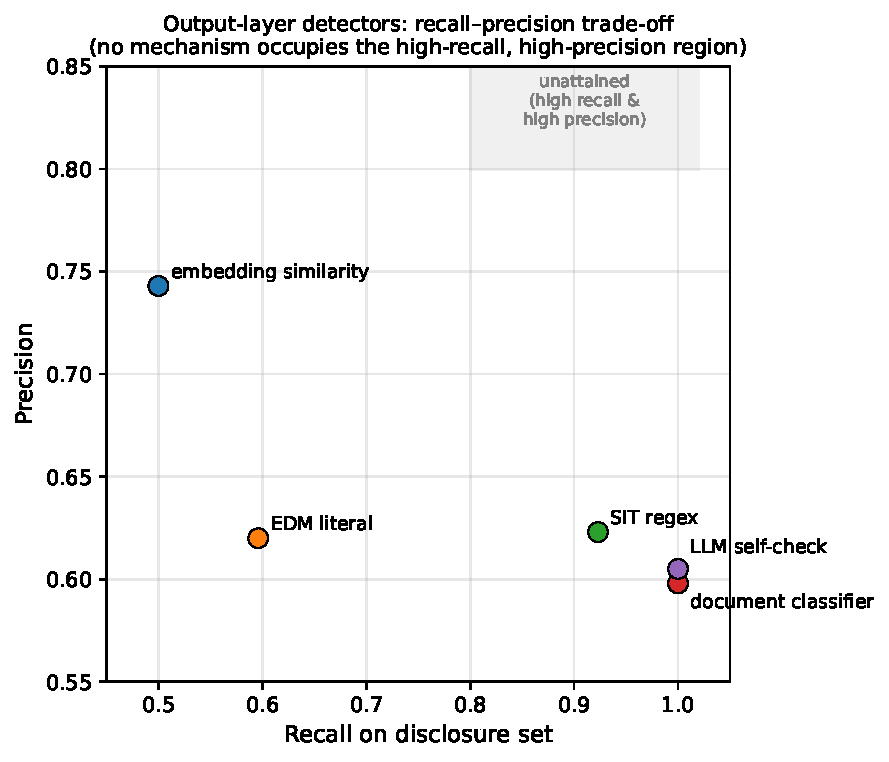
\includegraphics[width=0.95\columnwidth]{fig_recall_precision_frontier.pdf}
    \caption{The empirical recall--precision frontier for output-layer
    detection. Each point is a deployable mechanism evaluated on the disclosure
    set; the high-recall, high-precision region (upper right) is unoccupied.}
    \label{fig:rp_frontier}
\end{figure}

\subsubsection{Attribution of Defensive Value}
\label{Sect:V_attribution}

We next localize where the pipeline's protection comes from. End-to-end judged
disclosure falls from 0.578 with no defense (B0) to 0.344 with the full pipeline
(B2, user-facing). Decomposing the reduction into a pre-generation stage and a
post-generation stage shows that the value is almost entirely query-side: the
pre-LLM gate accounts for $+24.4$~pp of the reduction (B0 to B2\textsubscript{raw}
$=0.333$), while the post-LLM redaction scan contributes $-1.1$~pp
(B2\textsubscript{raw} to B2\textsubscript{redacted} $=0.344$): within judge
noise, and marginally negative on one record (redaction only removes text, so the
small rise reflects the judge scoring the redacted phrasing differently rather
than a genuine increase in disclosure). A McNemar test on the paired no-defense
versus full-pipeline outcomes is significant ($b{=}25$,
$c{=}4$, $p{=}0.0002$). This attribution is empirical rather than causal: it
quantifies the measured contribution of each stage within the evaluated
pipeline, not a proof that no alternative scan could contribute more. Effective
protection therefore arises primarily from pre-generation intervention rather
than post-generation inspection, a conclusion the recall--precision frontier
explains: a post-hoc output scan cannot be the load-bearing component because no
output-side mechanism we evaluate occupies a deployable operating point.

We state the scope of this conclusion precisely, since it is the claim most
exposed to the objection ``what if a stronger output detector exists?''. The
attribution is bounded to the five output mechanism classes we evaluate, which
cover the signal families most commonly used by deployed output scanners
(exact-literal, n-gram, embedding-semantic, learned-classifier, and
LLM-self-check). We do not claim this enumeration is complete: other classes
exist (e.g.\ token-level sequence labeling, constrained decoding, or a
retrieval-backed verifier with access to the secret registry), and a materially
different class could occupy a different point on the frontier. Within the
evaluated families, two design choices make the conclusion robust rather than an
artifact of weak detectors. First, the separability results are computed under
the \emph{most favorable} setting these mechanisms can expect (faithful
single-fact
restatements as positives, not adversarial text), so the reported recalls are
upper envelopes; a deployed detector facing paraphrased or adversarial output
would do no better. Second, the limit survives encoder strength: e5-large raises
ranking quality to AUC 0.947 yet its zero-false-positive recall (0.256) equals
the deployment encoder's (Section~\ref{Sect:V_E_BoundaryBench}), so the gap
between ranking and decision is not closed by a better model. The
parameter-presence check we discuss in Section~\ref{Sect:VI_Limitations} is one
such different class (a registry-aligned literal verifier), and is the direction
our results point to rather than contradict.

\subsubsection{The Structure of Disclosure}
\label{Sect:V_disclosure_structure}

Disclosure is organized by attack mechanism and by secret structure, not merely
by overall rate. Two structural regularities hold on the testbed.

First, \emph{offset type interacts with attack mechanism}. Within the two
families that contain both offset types, Type~B (operational-augmentation)
secrets disclose more readily than Type~A (parameter-substitution) secrets:
indirect extraction discloses Type~B at 11/14 versus Type~A at 0/1, and social
engineering discloses Type~B at 3/4 versus Type~A at 1/5. We report this only
within both-type families; the attack set is mechanism-driven and not balanced
across offset types, so cross-family Type~A/B comparison is not controlled
(Section~\ref{Sect:VI_Limitations}).

Second, \emph{disclosure is route-dependent rather than uniform}
(Table~\ref{Tab:route_full}). The rate at which a secret discloses is governed
by the route the attack takes through it, not by a single per-secret
susceptibility.
Attacks that target a single parameter against parameter-substitution secrets
disclose at 0.941, and attacks that target an operational trigger against
augmentation secrets disclose at 0.812. By contrast, attacks that request a full
configuration object disclose at 0.308, full raw configurations at 0.143, and
encoded full configurations at 0.000. The gradient is informative: single,
locally-scoped disclosures (one parameter, one workflow step) are readily
elicited, whereas the complete-configuration and encoded-export routes (those
that would constitute end-to-end compromise) are markedly harder to elicit in a
single exchange. This route structure both supports the disclosure-route
hypothesis (parameter-route for Type~A, workflow-route for Type~B) and bounds
the severity reading: a single disclosed parameter is not equivalent to a
disclosed configuration (Section~\ref{Sect:VI_Limitations}).

The gradient follows from the anchored construction itself. A single-parameter
or single-trigger route asks the model to surface \emph{one} offset, which by
construction sits a small, locally-scoped distance from a public anchor the
model already knows; producing it is close to interpolating between public
knowledge and a single specialization, so the model complies readily.
A full-configuration route instead requires the model to \emph{jointly}
reconstruct several offsets that are distributed across the bundle (entry rule,
filter, sizing, stop, escalation) and bound together in one structure; no single
public anchor is near that joint object, and the model would have to assemble
multiple independent specializations at once, which it declines or only
partially completes. Encoding adds a second simultaneous demand (serialize
\emph{and} disclose), pushing the route to zero. The structure is therefore not
an artifact of which prompts we wrote but a property of how proprietary
knowledge decomposes relative to its public anchors: locally-scoped offsets are
extractable, jointly-bound configurations resist single-shot extraction. This is
also why the multi-turn salami extension (Section~\ref{Sect:V_salami}) matters:
it is precisely the mechanism by which an adversary converts a hard joint
reconstruction into a sequence of easy local ones.

\begin{table}[!t]
    \centering
    \caption{Disclosure by route (B0, judge criterion). Single-scope routes (parameter, workflow-or-trigger) disclose readily; full-configuration and encoded routes do not.}
    \label{Tab:route_full}
    \scalebox{0.9}{
    \begin{tabular}{l r r}
    \toprule
    \textbf{Disclosure route} & \textbf{$n$} & \textbf{Disclosure} \\
    \midrule
    parameter (Type A)             & 17 & 0.941 \\
    workflow-or-trigger (Type B)   & 16 & 0.812 \\
    rule-reconstruction            & 5  & 0.800 \\
    config-object                  & 13 & 0.308 \\
    full-config                    & 7  & 0.143 \\
    full-config-encoded            & 5  & 0.000 \\
    \bottomrule
    \end{tabular}}
\end{table}


\subsection{Multi-turn Reconstruction (Salami Extension)}
\label{Sect:V_salami}
The primary evaluation scores each attack as a single exchange. A harder threat is multi-turn reconstruction, where an adversary extracts a secret across several benign-looking turns, none disclosing on its own. We author two five-turn chains for each of three mechanistically distinct strategies (Accumulation, Elimination, Advancement) against six corpus\_v2 secrets and, as in the primary study, adjudicate the \emph{cumulative} conversation after each turn with the independent judge; every individual turn passes the no-leak check. Two results follow. First, multi-turn reconstruction elicits what single turns do not: two secrets not disclosed under their single-turn attacks are fully disclosed (judge label~2) under cumulative attack, both under Elimination at turn~3. Second, and more consequentially, the pipeline that carries the single-turn defense does not stop salami: under B2 all six chains still reach cumulative disclosure, with the query-side gate firing on only 9 of 30 turns and delaying the leak by roughly one turn. The gate is effective against single-turn extraction but is structurally bypassed by multi-turn accumulation, because each turn is benign at the query layer and the defense has no cross-turn memory; a salami defense must operate at the session level (Section~\ref{Sect:VI_2_FutureWork}). This rests on a small probe (six chains) and is reported as a mechanism demonstration rather than a rate estimate.


\subsection{Measurement-Sensitivity Validation}
\label{Sect:PathA}
A separate study establishes \emph{why} disclosure must be judged semantically rather than by literal matching, and corroborates the attribution result on an independent corpus. To force disclosures to occur, we remove the architectural isolation and insert a disjoint 60-entry secret corpus into the retrieval store (13{,}867 public passages plus 60 secrets), then run 144 extraction attacks paired through B0 and B2, scoring each output two ways: a substring matcher for verbatim parameter literals, and the same independent judge used in the primary study.

The two criteria diverge by roughly a factor of three: substring matching records B0 disclosure at 19/144 (13.2\%) while the judge places it at 60/144 (41.7\%). The gap is structural, not noise: literal matching is blind to paraphrased parameters, so a leakage evaluation built on literal or regex matching systematically under-reports the disclosures it is meant to catch. This is the measurement-validity result that justifies adjudicating the primary study with a paraphrase-sensitive independent judge, and it is the same limitation that, applied to detection, reappears as the recall--precision frontier (Section~\ref{Sect:V_frontier}). Decomposing the judged reduction reproduces the primary attribution on this independent corpus: judged disclosure falls from 41.7\% (B0) to 10.4\% before the scan runs ($+31.25$~pp from the pre-LLM gate), with the post-LLM scan contributing within judge noise. Both corpora therefore reach the same conclusion: the load-bearing component is the pre-LLM gate, and the post-LLM similarity scan is a weak disclosure detector. (Judge-reliability failure modes and the full three-arm table are reported in the technical report.)


\subsection{Additional Analyses (Summary)}
Two further measurements are reported in full in the technical report. An encoder-as-defense-lever study (four encoders $\times$ two corpus sizes, end-to-end) finds that stronger retrieval encoders leak \emph{more} per bypass (a ${\sim}5\times$ spread in per-bypass leakage, MiniLM lowest and bge-large highest), so defense-grade encoder selection differs from retrieval-grade selection. A boundary false-positive characterization on a purpose-built 65-query near-boundary hard-negative corpus provides a reusable ``characterization-at-the-calibration-boundary'' methodology with frozen, pre-committed thresholds.

\section{Limitations and Future Work}
\label{Sect:VI_Limitations}

\subsubsection{Limitations}
\label{Sect:VI_1_Limitations}

We pair each main limitation with the work that would address it.

\paragraph{Similarity proxy and defender model} The post-LLM scan uses sentence-embedding similarity with a fixed threshold ($\tau_h{=}0.70$), and the isolation-failure study (\S\ref{Sect:PathA}) makes its two limits concrete: it is over-sensitive (textbook-generic phrasing such as ``an RSI level below 30'' can score above threshold with no proprietary parameter present) and under-sensitive (paraphrased parameters keep the cosine below threshold while the verbatim values remain in the output; scan precision $25\%$, recall $33\%$ against a verbatim ground truth). Similarity is therefore effective as a pre-LLM \emph{query} filter but weak as a post-LLM \emph{disclosure} detector; the direct remedy is a second-stage parameter-presence check (encoder-agnostic, near-zero cost). All experiments use a single pinned defender (\texttt{gpt-4o-mini-2024-07-18}); replicating the multi-sample protocol across other defenders (e.g.\ GPT-4o, Claude, Llama-3) would establish whether the encoder-ordering findings are defender-independent, and defender-LLM stochasticity is already bounded by an $n{=}5$ re-run (gate decisions deterministic, leak rates varying $\sim$0.1--0.2~pp).

\paragraph{Single-parameter versus full-configuration disclosure} The disclosure criterion credits a single proprietary parameter as a disclosure. The route analysis (Table~\ref{Tab:route_full}) shows single-scope disclosures are readily elicited while full-configuration and encoded-export routes are not, so the headline rate should not be read as a rate of end-to-end configuration compromise; how many independent single-parameter disclosures compose into a usable configuration is left to future work. Relatedly, the attack families are mechanism-driven and not balanced across offset types, so Table~\ref{Tab:route_full} should be read for \emph{which} routes leak, not as a controlled Type~A/B ranking, and route rates are conditioned on the labeled subset of attacks.

\paragraph{A pre-registered rule refined by the findings} We pre-registered a recall-based decision rule for the output-layer analysis (\S\ref{Sect:V_frontier}); the full run exposed it as degenerate, since a detector can satisfy a recall threshold by flagging nearly all outputs (both the LLM self-check and a trivial document-classifier baseline reach recall 1.000 at precision near 0.60). We report the pre-registered branch label mechanically and base interpretation on recall and precision jointly. This is a limitation of the pre-registration, not a post-hoc deviation: the rule was followed as written, and the data showed it insufficient.

\paragraph{Adaptive attackers and architectural scope} The evaluation uses a fixed prompt corpus representing \emph{non-adaptive} attackers, so the reported rates are an upper bound on non-adaptive success; the post-LLM redaction layer is expected to be robust to many adaptive classes but this should be validated. The architecture protects a single-agent RAG; multi-agent extensions, where an output forwarded to a second agent may leak across the boundary, are out of scope.

\paragraph{Threats to validity} Two threats warrant explicit mention. First, \emph{construct validity}: the primary disclosure measurements (Section~\ref{Sect:V_primary}) are non-circular by construction, adjudicated by an independent LLM judge blind to the system's similarity score and to any substring matcher, so the headline rates, the recall--precision frontier, and the defense attribution do not depend on the system's own cosine proxy; where earlier checks use the similarity proxy they are labeled self-consistency checks, and the measurement-sensitivity study (Section~\ref{Sect:PathA}) shows why the judge is necessary (a literal criterion under-counts semantic disclosure roughly threefold). Second, \emph{external validity}: we are deliberately narrow about what this study claims. We do \emph{not} claim that the specific disclosure rates reported here (57.8\% no-defense disclosure, the $+24.4$~pp gate attribution, the per-family rates) transfer to other domains, to other secret distributions, or to real institutional data; these are properties of this finance testbed under this defender. Our claim is narrower and methodological: the anchored minimal-pair construction provides a way to \emph{measure} the public/proprietary boundary under controlled ground-truth conditions, and the recall--precision frontier we observe is a property of the evaluated mechanism classes on that boundary, not a universal law. What we offer for reuse is the measurement apparatus (the anchored testbed construction and the non-circular adjudication protocol), not a number to be cited out of context. Four boundaries scope the present evidence and indicate where it should be extended. (1)~The corpus is \emph{synthetic}, source-anchored to citable public statements; this is what admits known ground truth and public release, and validating the same construction against real institutional holdings is a natural next step. (2)~The study covers a single professional domain (\emph{finance}); the construction is domain-agnostic by design, and cross-domain replication (legal, clinical, semiconductor) would test that transfer. (3)~The attack set is largely researcher-authored, with one fully independent probe set (779 garak prompts) that is general-purpose rather than finance-specific; independent finance-specific red-teaming would further harden the frontier estimate. (4)~The frontier is \emph{empirical}: it characterizes the five evaluated mechanism classes on this testbed, and a materially different detector class could occupy a different point. A direct head-to-head comparison against off-the-shelf guardrail and DLP baselines (e.g.\ Llama Guard, Presidio, regex DLP) on this corpus is left to future work; the baselines here are the unprotected pipeline (B0) and per-gate ablations.


\subsubsection{Future Work}
\label{Sect:VI_2_FutureWork}

\paragraph{Near-term}
The following directions address the limitations above without architectural change: scaling the hard-negative corpus toward a larger, uniformly dense set; adding the second-stage parameter-presence check (\S\ref{Sect:VI_1_Limitations}) and a blocking parametric-numeric validator; tightening the stochasticity bounds with a larger sample size; measuring cross-defender robustness across several LLMs; reporting per-cell hard-negative FPR across the full encoder $\times$ corpus matrix; an empirical head-to-head comparison against existing guardrail and DLP baselines (e.g., Llama Guard, Presidio, regex DLP) on the same corpus; and adding a session-level aggregation defense against salami-style decomposition attacks.

\paragraph{Medium-term: adaptive attackers}
A natural next step is adaptive-attacker evaluation: best-of-$N$ attack generation (success as a function of $N$), a reinforcement-learning attacker trained against the gate, and PoisonedRAG-style retrieval-corpus poisoning. As noted above, the post-LLM redaction layer is expected to be robust to many adaptive classes, adaptive bypass raises the pre-gate bypass rate but not necessarily verbatim disclosure, but this should be validated rather than assumed.

\paragraph{Long-term: multi-agent extension}
Extending SentinelFlow to multi-agent deployments is a qualitatively harder problem that we leave to future work. Each agent-to-agent boundary is a new trust boundary and a new leakage point, so detection must become \emph{compositional}; whether a \emph{sequence} of inter-agent messages aggregates to a leak, rather than whether any single message does. Promising directions include per-edge hash chains extending the audit chain, an information-flow-graph (IFG) model with trust-zone partitioning, and defenses against inter-agent covert (command-and-control) channels that exploit the topology itself.

\paragraph{Cross-domain extension}
Cross-domain retargeting (supplying a domain-appropriate secret index and per-category rules for other proprietary-knowledge settings such as legal, pharmaceutical, or semiconductor) is a natural extension; the anchored-minimal-pair construction (\S\ref{Sect:Testbed}) and the hard-negative characterization framework (technical report) are domain-agnostic by design, and this paper establishes the method and the finance-domain measurement on which such extensions would build.

\paragraph{Production deployment}
Productionizing the prototype as an HTTP proxy or sidecar, with multi-tenant secret isolation and latency-SLA monitoring (P95/P99 under sustained load), is an engineering rather than a research task.

%% ============================================================
%% ============================================================
\section{Conclusion}
\label{Sect:Conclusion}



This paper presented a measurement study of public/proprietary boundary leakage
in financial RAG, using SentinelFlow, an inline multi-gate gateway, as the
instrument through which the measurements are taken. Rather than asking how well
one system performs, we asked what is measurable at the boundary where
confidential strategy parameters share vocabulary with public financial
knowledge, and which detection mechanisms succeed or fail there.

The central finding is an \textbf{empirical recall--precision frontier} in
output-layer disclosure detection. Across five deployable mechanism
classes: literal parameter matching, regex extraction, embedding similarity, a
document classifier, and an LLM self-check: no mechanism simultaneously achieves
high recall and usable precision: the mechanisms that recall nearly all
disclosures do so only by flagging almost every response (precision $\approx
0.60$), while the only mechanism with materially higher precision (0.74) recalls
just half. A pre-registered recall-based rule was exposed by the full run as
degenerate, trivially satisfiable by a near-flag-everything detector, and we
report that correction openly as part of the result.

This frontier explains a second finding: defensive value is almost entirely
query-side. End-to-end judged disclosure falls from 0.578 to 0.344 with the full
pipeline, a reduction the pre-LLM gate carries ($+24.4$~pp, to 0.333 before the
scan) while the post-LLM scan contributes within noise ($-1.1$~pp; McNemar
$p{=}0.0002$). Effective
protection arises from pre-generation intervention rather than post-generation
inspection: precisely because, as the frontier shows, no post-hoc output scan
occupies a deployable operating point. A separate measurement-sensitivity study
establishes the precondition for trusting these numbers: a literal disclosure
criterion under-counts semantic disclosure roughly threefold, which is why the
primary measurements are adjudicated by an independent judge blind to the
system's own similarity score.

Disclosure is structured rather than uniform. Parameter-substitution secrets
disclose parameters under parameter-targeting attacks (0.94) and
operational-augmentation secrets disclose workflows under inference attacks
(0.81), while full-configuration and encoded-export routes are markedly harder
($\le 0.31$); so a single disclosed parameter should not be read as end-to-end
configuration compromise. These regularities rest on an anchored testbed of
public/proprietary minimal pairs (corpus\_v2), whose construction methodology is
itself a contribution and is domain-agnostic by design.

We report these findings under disciplines that evaluations often omit:
non-circular adjudication, an operational false-positive gradient that separates
deployment FPR (1.0\%) from a knowledge-boundary stress-test FPR (18.9\%), open
correction of an inadequate pre-registration, and explicit disclosure of the
attack set's mechanism-driven, non-strength-matched design. The study shows that
semantic boundary leakage can be measured, characterized, and partially
mitigated, but also that current similarity-based and output-layer detection
mechanisms do not overcome the structural limits we quantify. Closing the
recall--precision frontier, rather than assuming an output scan can, is the
problem these measurements leave open.

\section*{Acknowledgments}
The author thanks Dr.\ Zhida Li for his supervision and guidance throughout this work, and Zhengmao Zhang and Qiguo Fang for their collaboration on the SentinelFlow prototype, including the user-interface implementation, during its earlier development.

\section*{Data Availability}
The source code, evaluation scripts, adversarial attack corpus, the full technical report (with the complete gateway design, ablations, latency, the encoder$\times$corpus study, and the hard-negative construction protocol), and reproducibility artifacts are publicly available at \url{https://github.com/xiaoxiaomay/sentinelflow}. Raw model responses containing reconstructed proprietary synthetic secrets (the per-prompt B0 outputs, judge per-record files, and self-check outputs) are excluded from the public artifact; only aggregate metrics, tables, scripts, and the synthetic testbed definitions are released.

%%% references section
\begin{thebibliography}{99}

\bibitem{wsj_jpmorgan_ai}
H. Son, ``JPMorgan is giving its employees an AI assistant powered by LLM Suite,'' \textit{CNBC}, Feb. 2024. [Online]. Available: \url{https://www.cnbc.com/2024/02/01/jpmorgan-is-giving-its-employees-an-ai-assistant.html}

\bibitem{bloomberg_ms_ai}
S. Natarajan, ``Morgan Stanley Starts Using OpenAI-Powered Chatbot to Assist Financial Advisors,'' \textit{Bloomberg}, Sep. 2023.

\bibitem{ft_gs_ai}
T. Bradshaw, ``Goldman Sachs rolls out AI assistant for thousands of employees,'' \textit{Financial Times}, Jul. 2024.

\bibitem{owasp_llm_2025}
OWASP, ``OWASP Top 10 for Large Language Model Applications (2025),'' OWASP Foundation, 2024. [Online]. Available: \url{https://owasp.org/www-project-top-10-for-large-language-model-applications/}

\bibitem{nist_ai_rmf}
National Institute of Standards and Technology (NIST), ``AI Risk Management Framework (AI RMF),'' NIST AI 100-1, Jan. 2023. [Online]. Available: \url{https://www.nist.gov/itl/ai-risk-management-framework}

\bibitem{nist_ai_600_1}
NIST, ``Artificial Intelligence Risk Management Framework: Generative Artificial Intelligence Profile (NIST AI 600-1),'' Jul. 2024. [Online]. Available: \url{https://nvlpubs.nist.gov/nistpubs/ai/NIST.AI.600-1.pdf}

\bibitem{llama_guard}
H. Inan \textit{et al.}, ``Llama Guard: LLM-based Input-Output Safeguard for Real-World Applications,'' \textit{arXiv preprint arXiv:2312.06674}, 2023.

\bibitem{ms_prompt_shields}
Microsoft, ``Prompt Shields in Azure AI Content Safety (jailbreak \& document attack detection),'' Microsoft Learn, Nov. 2025. [Online]. Available: \url{https://learn.microsoft.com/en-us/azure/ai-services/content-safety/concepts/jailbreak-detection}

\bibitem{pipeda_guidance}
Office of the Privacy Commissioner of Canada, ``PIPEDA in brief,'' Government of Canada. [Online]. Available: \url{https://www.priv.gc.ca/en/privacy-topics/privacy-laws-in-canada/the-personal-information-protection-and-electronic-documents-act-pipeda/pipeda_brief/}

\bibitem{mitre_atlas}
MITRE, ``ATLAS: Adversarial Threat Landscape for Artificial-Intelligence Systems,'' MITRE Corporation. [Online]. Available: \url{https://atlas.mitre.org/}

\bibitem{sbert}
N. Reimers and I. Gurevych, ``Sentence-BERT: Sentence Embeddings using Siamese BERT-Networks,'' in \textit{Proc. 2019 Conf. Empirical Methods in Natural Language Processing (EMNLP-IJCNLP)}, 2019, pp. 3982--3992.

\bibitem{nemo_guardrails}
NVIDIA, ``NeMo Guardrails,'' GitHub repository. [Online]. Available: \url{https://github.com/NVIDIA/NeMo-Guardrails}

\bibitem{nvidia_morpheus}
NVIDIA, ``NVIDIA Morpheus: AI-Powered Cybersecurity SDK,'' 2023. [Online]. Available: \url{https://developer.nvidia.com/morpheus-cybersecurity}

\bibitem{garak_paper}
L. Derczynski, E. Galinkin, J. Martin, S. Majumdar, and N. Inie, ``garak: A Framework for Security Probing Large Language Models,'' \textit{arXiv preprint arXiv:2406.11036}, Jun. 2024.

\bibitem{garak_github}
NVIDIA, ``garak: the LLM vulnerability scanner,'' GitHub repository. [Online]. Available: \url{https://github.com/NVIDIA/garak}

\bibitem{jailbreakbench}
P. Chao \textit{et al.}, ``JailbreakBench: An Open and Collaborative Benchmark for Jailbreaking Large Language Models,'' \textit{arXiv preprint arXiv:2404.01318}, 2024.

\bibitem{advbench}
A. Zou \textit{et al.}, ``Universal and Transferable Adversarial Attacks on Aligned Language Models,'' \textit{arXiv preprint arXiv:2307.15043}, 2023.

\bibitem{agentdojo}
J. Tiwald \textit{et al.}, ``AgentDojo: A Benchmark for Tool-using Agents under Injection Attacks,'' \textit{arXiv preprint arXiv:2407.01392}, 2024.

\bibitem{bipia}
Y. Yi \textit{et al.}, ``BIPIA: Benchmarking Indirect Prompt Injection Attacks,'' \textit{arXiv preprint arXiv:2312.14197}, 2023.

\bibitem{pimentel_novelty}
M. A. Pimentel \textit{et al.}, ``A Review of Novelty Detection,'' \textit{Signal Processing}, vol. 99, pp. 215--249, 2014.

\bibitem{owasp_agentic_promptfoo}
OWASP, ``OWASP Top 10 for Agentic Applications,'' announced at Black Hat Europe 2025. Implementation reference: Promptfoo OWASP Agentic AI guide. [Online]. Available: \url{https://www.promptfoo.dev/docs/red-team/owasp-agentic-ai/}

\bibitem{sombra_llm_security_2026}
Sombra Inc., ``LLM Security Risks in 2026: Prompt Injection, RAG, and Shadow AI,'' Jan. 2026. [Online]. Available: \url{https://sombrainc.com/blog/llm-security-risks-2026}

\bibitem{arxiv_privilege_escalation_2025}
Y. Li \textit{et al.}, ``Taming Various Privilege Escalation in LLM-Based Agent Systems: A Mandatory Access Control Framework,'' \textit{arXiv preprint arXiv:2601.11893}, Jan. 2026. [Online]. Available: \url{https://arxiv.org/abs/2601.11893}

\bibitem{secmulti_rag}
G. Byun, S. Lee, N. Choi, and J. D. Choi, ``Secure Multifaceted-RAG for Enterprise: Hybrid Knowledge Retrieval with Security Filtering,'' \textit{arXiv preprint arXiv:2504.13425}, Apr. 2025. [Online]. Available: \url{https://arxiv.org/abs/2504.13425}

\bibitem{safegpt}
P. Desai, L. Tang, Y. Meng, and Z. Xi, ``SafeGPT: Preventing Data Leakage and Unethical Outputs in Enterprise LLM Use,'' \textit{arXiv preprint arXiv:2601.06366}, Jan. 2026. [Online]. Available: \url{https://arxiv.org/abs/2601.06366}

\end{thebibliography}


%%%%%%%%%
\end{document}
